% modify the fontscale parameter to make everything slighly bigger or smaller.
\documentclass[portrait,a0paper,fontscale=0.25]{baposter}

\usepackage[czech]{babel}

\usepackage[utf8]{inputenc}
\usepackage[T1]{fontenc}
\usepackage{svg}
\usepackage{enumitem}


% FONT CHOICES
% Posters do not need to be PDF/A; you can choose any relatable font from the
% TeX font catalogue without much risk. Sans-serif fonts are suggested for the
% posters; see https://tug.org/FontCatalogue/sansseriffonts.html
%\usepackage[sfdefault]{Fira Sans}
%\usepackage[default]{droidsans}
%\usepackage[math]{iwona}
\usepackage[defaultfam]{montserrat}
%\usepackage{cmbright}
%\usepackage{yfonts}\renewcommand{\familydefault}{\frakdefault}

\usepackage{color}
\usepackage{graphicx}
\usepackage{amssymb,amsmath}
\usepackage[export]{adjustbox} %allows using valign with \includegraphics

\renewcommand{\arraystretch}{1.5}

\usepackage{enumitem}
\setlist{itemsep=1pt}

\usetikzlibrary{positioning}

% A WORD ABOUT COLORS
%
% This template is prepared with a relatively neutral gray background that
% gives decent box borders (with white and darker gray), does not clash with
% many colors (except for violet-brown and other mushroomish colors, perhaps)
% and gives a lot of space for highlighting stuff.
%
% Generally, other color variations are good too; there are no strict rules on
% the colors. Good choices include:
%
% - white backgrounds and differentiation of box headers by color (see
%   headerFontColor)
%
% - various slightly tinted backgrounds (try red!10 instead of black!3)
% 
% - dark backgrounds
%
% Keep in mind:
% - The normal "informative" text and figures should be DARK on LIGHT
%   background, not the other way around.
%
% - Do not mix too many color hues together. Most hues have their widely
%   accepted meaning (green: good result, red: problem, blue: information,
%   yellow: highlighter, brown: serious problem, violet: something really
%   weird/interesting/magic, depending on the shade).

\begin{document}

    \color{black!80} % default font color
    \begin{poster}{grid=false,
        eyecatcher=true,
        background=plain,
        bgColorOne=black!3, % background color
        columns=2,
        headerborder=none,
        textborder=none,
        headershape=rounded,
        headershade=plain,
        boxshade=plain,
        boxColorOne=white,
        headershade=plain,
        headerColorOne=black!15, % box header background color
        headerFontColor=black,
        boxpadding=4mm
    }%
    {
\includegraphics[height=7em]{logos/mff-black}}
    {Platforma pro monitorování mentálního zdraví}
    {\vspace{1ex} Patrik Trefil}
    {
\includegraphics[height=7em]{logos/uk-red}}


%
% LEFT COLUMN
%

        \begin{posterbox}[column=0,name=intro]{úvod}
            Tato práce vznikla z motivace zlepšit kvalitu poskytované zdravotní péče v oblasti duševního zdraví za pomoci digitálních technologií.
            Při léčbě duševních potíží se často využívají domácí úkoly papírové formy, které jsou následně manuálně vyhodnocovány terapeuty.
            Digitalizací procesu spolupráce lze zajistit efektivnější spolupráci mezi terapeuty a pacienty a automatizovaný sběr dat o pacientech.
            Získaná data lze využít pro sledování vývoje stavu pacientů a také pro výzkum.

            V době analýzy existujících řešení nebylo nalezeno žádné řešení pro online spolupráci terapeutů a pacientů.

            Tato práce byla vytvořena ve spolupráci s Národním ústavem duševního zdraví, který poskytl svou expertízu a zkušenosti v oblasti duševního zdraví.
        \end{posterbox}

        \begin{posterbox}[column=0, name=goals, below=intro]{návrh řešení}
            Na základě analýzy požadavků zadavatele byla navržena webová aplikace s těmito hlavními funkcemi:

            \begin{itemize}
                \item Drag and drop editor pro vytváření komplexních formulářů
                \item Zadávání úkolů pacientům/účastníkům studie terapeuty/výzkumníky
                \item Základní analýza sesbíraných dat v aplikaci a možnost exportu
            \end{itemize}

            Aplikace využívá architekturu typu klient-server.
            Na obrázku níže je zjednodušeně znázorněn návrh řešení.

            \begin{center}
                \includesvg[width=0.9\linewidth]{img/architecture.drawio}
            \end{center}

            Mezi hlavní kvalitativní požadavky ústavu patřila snadná rozšiřitelnost aplikace o další formy spolupráce a možnost provozu aplikace na vlastní infrastruktuře.
            Tyto požadavky byly adresovány vhodným rozdělením aplikace na komponenty a využití Docker pro snadné nasazení.
        \end{posterbox}

%
% FOOTER
%

%        \begin{posterbox}[column=0, span=2, name=footer, below=something2,
%            textborder=none, headerborder=none, boxheaderheight=0pt,
%            boxColorOne=black!3]{}
%            If some institute/grant/department sponsored the work, put an acknowledgement here.
%        \end{posterbox}

%
% RIGHT COLUMN
%
% It is usually best to fill most of the poster with your results and
% conclusions. Again, use simple annotated pictures wherever possible. Plots
% with measurements are perfect, tables are also good.
%

        \begin{posterbox}[column=1, name=impl]{implementace}
            Aplikace využívá existující open-source software Form.io pro správu formulářů a uživatelů.
            Ostatní části aplikace byly vyvinuty v jazyce TypeScript s využitím frameworku NextJS\@.
            Komunikace mezi serverem a klientem probíhá pomocí \textit{remote procedure call} knihovny.
            Komunikace mezi serverem a databází probíhá pomocí \textit{object relational mapping} knihovny.
            Na obrázku níže je zobrazena obrazovka pro správu úkolů z pohledu terapeuta.

            \begin{center}
                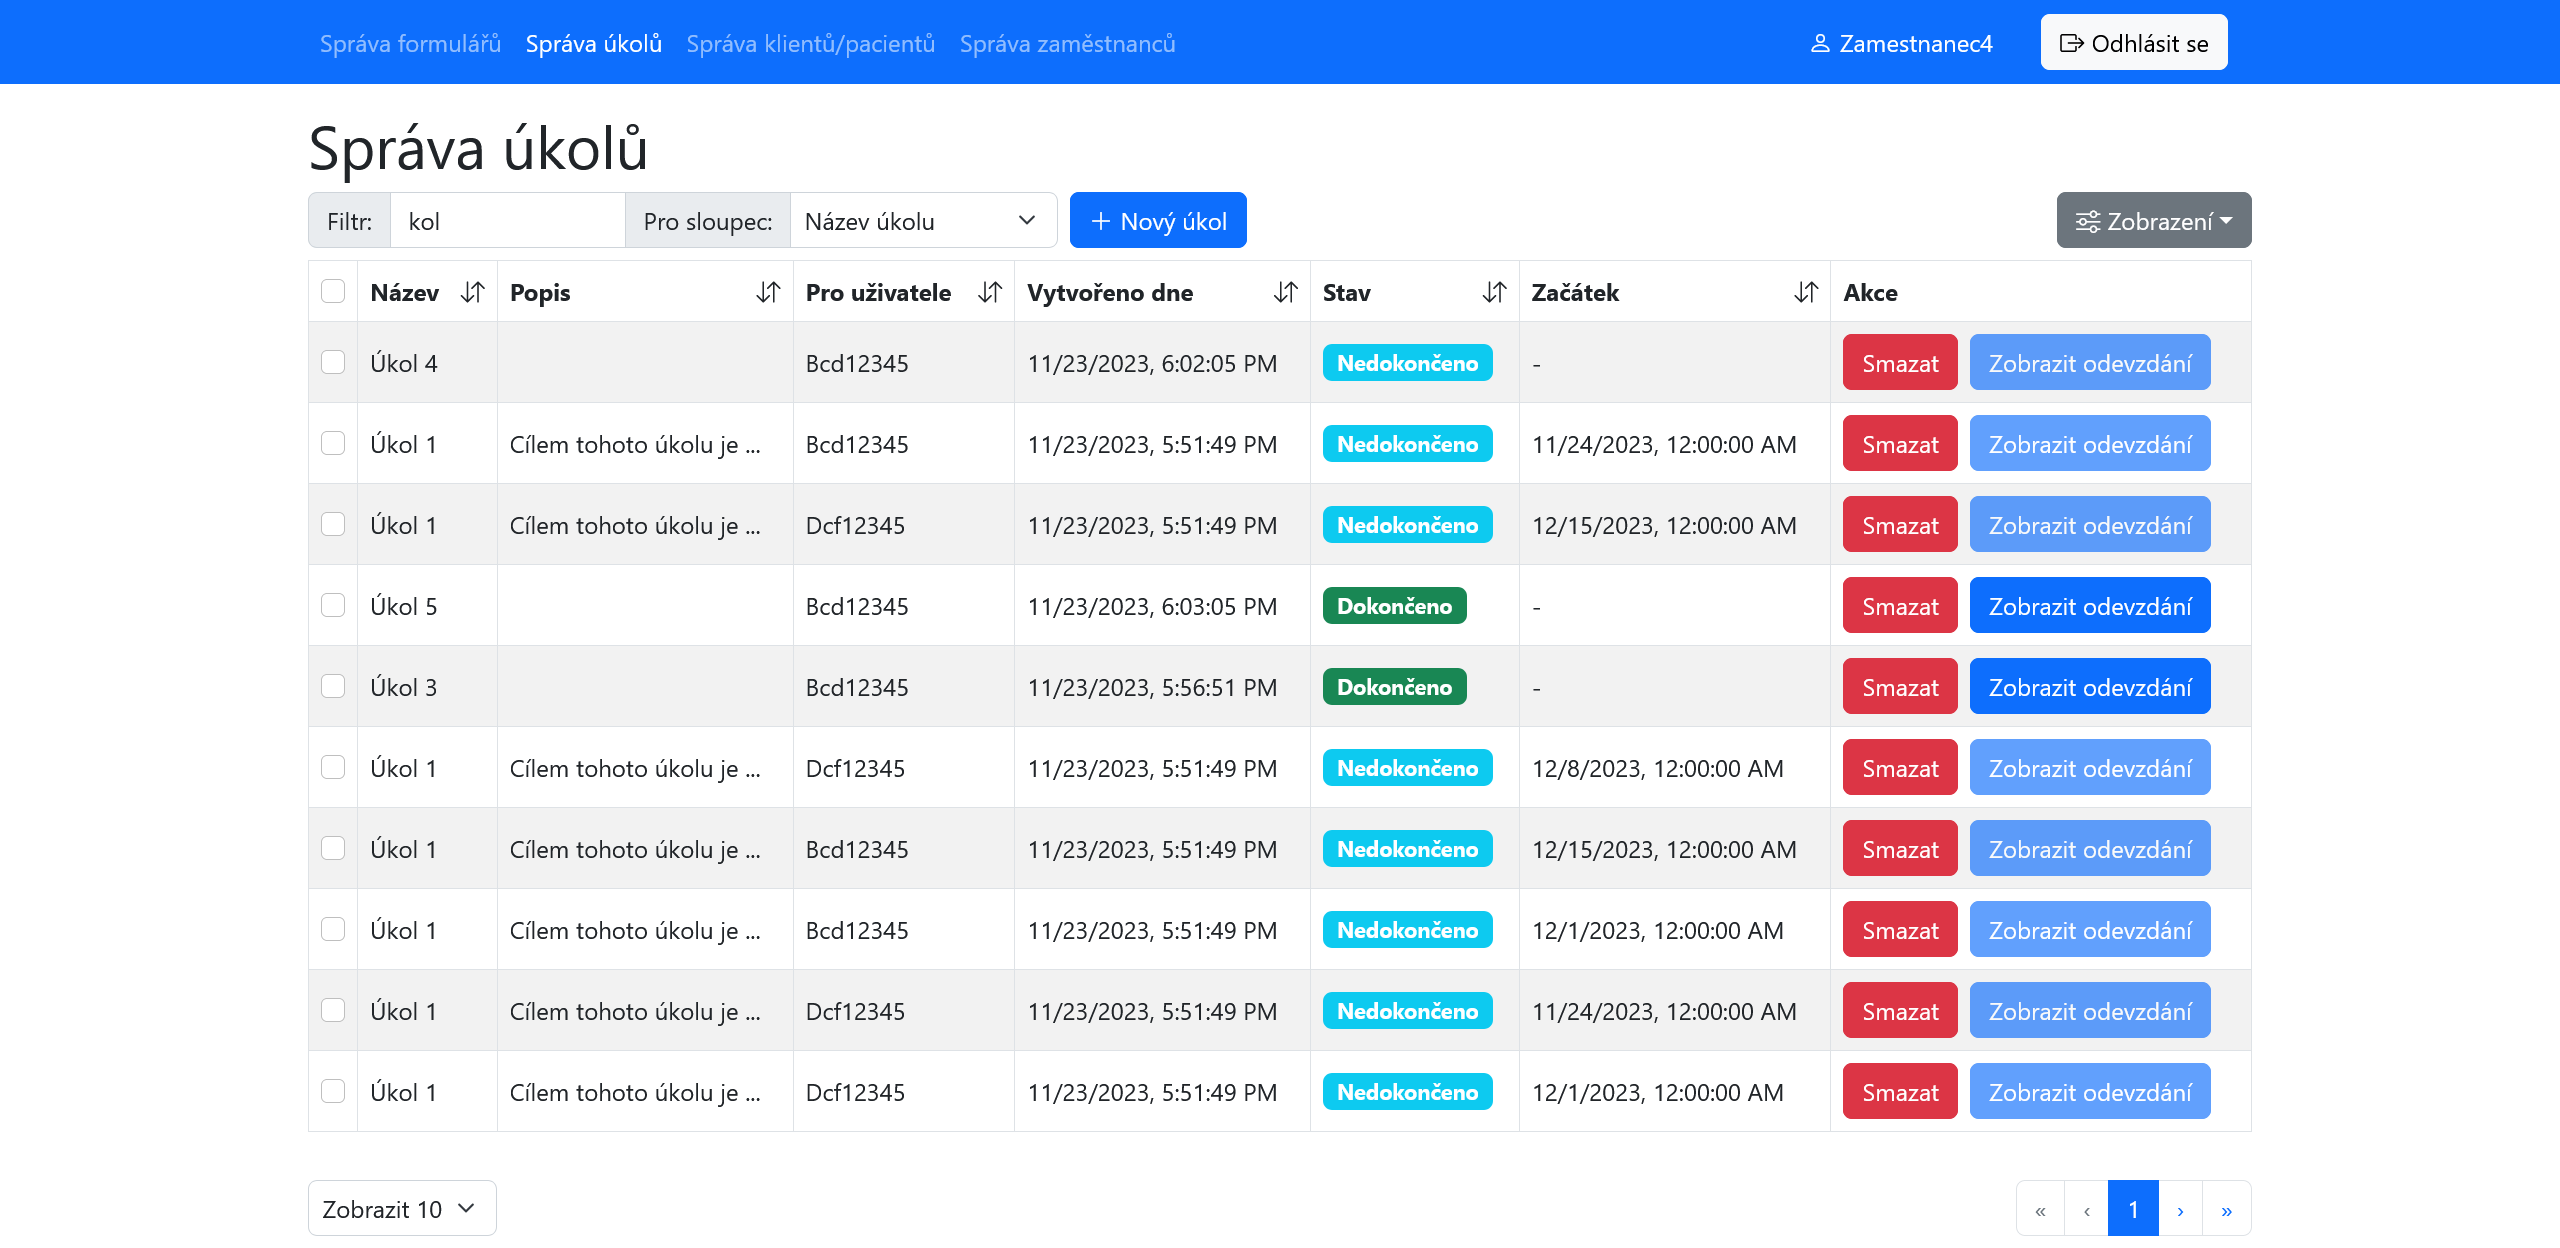
\includegraphics[width=\linewidth]{img/sprava-ukolu}
            \end{center}
        \end{posterbox}

        \begin{posterbox}[column=1, name=testing, below=impl]{testování}
            Serverová část aplikace je testována pomocí automatizovaných unit testů.
            Testujeme pouze veřejné rozhraní všech modulů.
            Objekt fungující jako proxy databáze byl nahrazen mock objekty.
            V tabulce níže je zobrazeno pokrytí serverové části automatizovanými unit testy.
            \begin{center}
                \begin{tabular}{c|c|c|c}
                    \textbf{Výrazy} & \textbf{Větve} & \textbf{Funkce} & \textbf{Řádky} \\
                    \hline
                    90.85 \%        & 72.91 \%       & 100 \%          & 90.85 \%       \\
                \end{tabular}
            \end{center}
        \end{posterbox}

        \begin{posterbox}[column=1, name=conclusion, below=testing]{shrnutí}
            Vyvinuli jsme plně funkční webovou aplikaci, která splňuje všechny požadavky zadavatele a je připravena do produkce.
            Vyvinůtý software je open-source a dostupný na platformě GitHub.
            Možné navazující práce:
            \begin{itemize}
                \item Přidání interaktivních vzdělávacích her nebo cvičení pro zvýšení motivace pacientů ke spolupráci
%                \item Přidání možnosti zasílání zpráv mezi terapeuty a pacienty pro řešení akutních potíží, či nejasností v zadaných úkolech
                \item Přidání schopnosti systému sledovat chování uživatele v průběhu vyplňování dotazníků
            \end{itemize}
        \end{posterbox}

        \begin{posterbox}[column=1, name=information, below=conclusion]{informace}
            Kontakt: patrik.trefil@gmail.com

            \vspace{2mm}

            Vedoucí bakalářské práce: Mgr.\ Petr Škoda, Ph.D., Katedra softwarového inženýrství
        \end{posterbox}

    \end{poster}
\end{document}
